%!TEX root = ../dokumentation.tex

% Inhalt 1:1 von Christian Buss übernommen

\chapter{Oberflächenprogrammierung}
Eine weitere Anforderung der Studienarbeit stellt die Visualisierung des gemessenen Gegenstandes dar. Dies wurde in Form eines Dialoges umgesetzt. Dazu wurden im Vorfeld Recherchen durchgeführt um die beste Komptabilität vom Dialog mit dem Raspberry Pi zu sicherzustellen. Mit Qt programmierte Dialoge habe ein gute Kommunikation mit dem Raspberry Pi. Infolgedessen wurde auf einer virtuellen Maschine ein Linux-Betriebssystem installiert, da auf dem Raspberry Pi Linuxbasierte Betriebssysteme sehr gut laufen. Auf diesem Betriebssystem wurde die Entwicklungssoftware Qt-Creater installiert. Die Software benutzt die Qt-Bibliothek, eine C++-Klassenbibliothek für die Programmierung von grafischen Benutzeroberflächen. 
Für den Dialog wurde zuerst ein einfacher Dialog angelegt. Auf diesem wird mithilfe von Zeichen-Events ein Raster gezeichnet das später zu Orientierung dienen soll. Zusätzlich werden drei Buttons eingefügt:
\begin{itemize}
	\item einer zum Schließen des Fensters
	\item einer zum Lokalisieren der Sensoren
	\item einer zum Starten der Messung.
\end{itemize}
Beim Klick auf den Lokalisierungs-Button wird ein Signal an die Sensoren gesendet welche dann den Abstand zueinander zurückgeben. Auf dieser Grundlage werden die jeweiligen Positionen ermittelt Dabei werden zwei der Sensoren auf bestimmte Koordinaten festgesetzt um die dritte Sensorposition besser bestimmen zu können. Die Abstände zwischen den Sensoren bilden die Seiten des Dreieck (Siehe Abbildung 1), dadurch kann dann der Winkel Alpha berechnet werden. Mit diesem Winkel und der Seite b kann die Höhe h berechnet werden. Jetzt kann der Satz des Phytagoras angewendet werden um $c_2$ zu berechnen. Dann muss nur noch h auf die y-Koordinaten und $c_2$ auf die x-Koordinaten addiert werden.
\begin{figure}
	\centering
	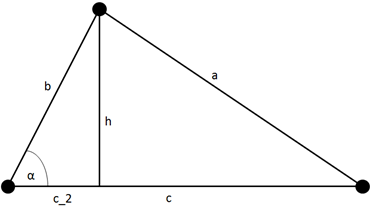
\includegraphics[scale=1]{images/gui/01.png}
	\caption{Berechnung der Sensorenpostion} \label{img:gui1}
\end{figure}

Sobald die Abstände bekannt sind werden die Positionen in dem Raster angezeigt. Da das Raster aus 16 Kasten besteht muss ein bestimmter Maßstab angegeben, dieser wird mittels der Abstände der Sensoren zueinander berechnet und neben einem Kasten zusätzlich dargestellt.\\
Mit betätigen des Buttons zum Starten der Messung wird ein Befehl an die Sensoren gesendet, diese geben dann einen Abstand zum Gegenstand zurück. Mit diesen Abständen wird eine Berechnung durchgeführt um die korrekte Position des Gegenstandes zu ermitteln. Die Abstände zum Gegenstand teilen das Dreieck nochmals in drei kleinere Dreiecke auf. Im nächsten Schritt werden die Winkel zum Ursprung berechnet, dadurch lässt sich die Steigung berechnen. Die Steigung sowie ein Punkt eines Sensors wird in die Geradengleichung eingesetzt und es kann der Startpunkt auf der Y-Achse berechnet werden. Somit kann die Geradengleichung aufgestellt werden. Dies wird für jeden Abstand durchgeführt, damit können durch das Gleichsetzten zweier Geradengleichungen der Schnittpunkt dieser ermittelt werden. Durch zweimaliges Wiederholen werden drei Schnittpunkte ermittelt, diese werden verglichen wenn die Abweichungen vernachlässigbar klein sind wird der Gegenstand im Raster angezeigt.
\begin{figure}[H]
	\centering
	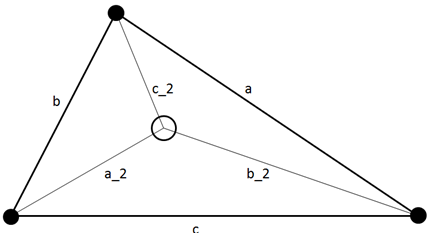
\includegraphics[scale=1]{images/gui/02.png}
	\caption{Berechnung der Position des Gegenstandes} \label{img:gui2}
\end{figure}

Wenn die Berechnung durchgeführt worden ist wird ein Kreis in das Raster gezeichnet um den Gegenstand zu symbolisieren. In Abbildung 3 zu sehen ist der Dialog.\\
Dieser Dialog wird dann auf dem Raspberry Pi gestartet und von diesem aus bedient und benutzt. Zu diesem Zweck wurde auf dem Raspberry Pi das Betriebssystem Rasbian installiert da dieses sehr einfach zu bedienen ist. Sobald der Raspberry Pi gestartet und an einen Bildschirm angeschlossen ist kann der Dialog einfach gestartet werden.
%TODO Seite drehen
\begin{figure}
	\centering
	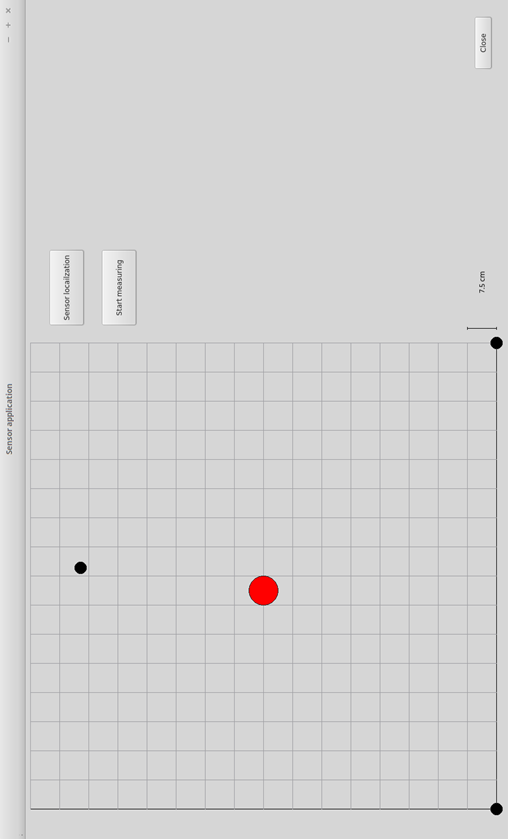
\includegraphics[width=(\textwidth)]{images/gui/03.png}
	\caption{Dialog zur Darstellung der Sensoren und des Gegenstandes} \label{img:gui3}
\end{figure}
